\begin{tabular*}{7in}{l@{\extracolsep{\fill}}r}
\textbf{\huge Arun Dunna} & \textbf{\today} \\
Research Assistant & \href{mailto:adunna@cs.umass.edu}{adunna@cs.umass.edu} \\
MS/PhD Student & \href{https://adunna.me}{https://adunna.me} \\
 & (404) 477-8660 \\
\end{tabular*}
\\

\resheading{Personal Information}


\begin{minipage}{.49\textwidth}
\begin{itemize}
\item[--] \textbf{Date of Birth:} April 18, 1998 \vspace{-6pt}
\item[--] \textbf{Gender:} Male \vspace{-6pt}
\item[--] \textbf{Nationality:} United States \vspace{-6pt}
\item[--] \textbf{Marital Status:} Single \vspace{-6pt}
\end{itemize}
\end{minipage}
\begin{minipage}{.49\textwidth}
  \flushright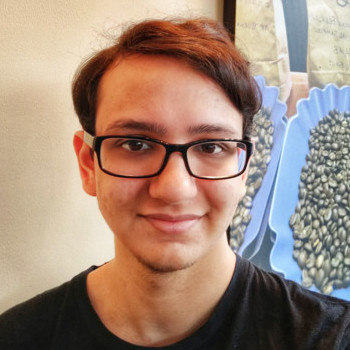
\includegraphics[scale=0.33]{me-small-square.jpg}
\end{minipage}

\resheading{Research Interests}

Networks, network measurement, network security, censorship and censorship circumvention, and digital privacy. Applications and influences of the listed areas to/on economics, politics, and social behaviors.

\resheading{Education}

\begin{itemize}

\item[]

	\ressubheading{University of Massachusetts Amherst}{Amherst, MA}{Ph.D. Computer Science}{Sep. 2019 -- TBD}

  \begin{itemize}
		\resitem{Advisor: Phillipa Gill}
    \resitem{Notable Courses: Research Methods for Empirical Computer Science (CS 691DD), Internet Law and Policy (CS 690L), Advanced Networks (CS 653), Advanced Natural Language Processing (CS 685)}
	\end{itemize}

\item[]

	\ressubheading{University of Massachusetts Amherst}{Amherst, MA}{M.S. Computer Science}{May 2018 -- Dec. 2020}

  \begin{itemize}
		\resitem{Advisor: Phillipa Gill}
    \resitem{Notable Courses: Advanced Algorithms (CS 611), Affective Computing (CS 527), Information Assurance (CS 660), Neural Networks (CS 682), System Defense (CS 590A)}
	\end{itemize}

\item[]

	\ressubheading{University of Massachusetts Amherst}{Amherst, MA}{B.S. Computer Science, Minor: Mathematics}{Sep. 2016 -- May 2018}

  \begin{itemize}

	\resitem{Notable Courses: Machine Learning (CS 589), Detecting Interference in Networks (CS 690B), Artificial Intelligence (CS 383), Financial Mathematics (M 537)}

	\end{itemize}

\end{itemize}

\newpage

\resheading{Research}

\begin{itemize}

\item[]

	\ressubheading{Calipr Lab}{Amherst, MA}{Advisor: Phillipa Gill}{Jan. 2017 -- Current}

  \begin{itemize}
    \resitemtwo{\textbf{Demonetized: Looking at the Black-box of YouTube}}{Jan. 2019 -- Current}
    \resitemtwo{\textbf{Investigating the Censorship of the IPv6 Web}}{Jan. 2019 -- May 2019}
    \resitemtwo{\textbf{Applying AS Hegemony to Tor}}{Nov. 2018 -- Current}
    \resitemtwo{\textbf{China's Tor-Resilient Infrastructure}}{Aug. 2018 -- Aug. 2019}
    \resitemtwo{\textbf{Analyzing China's Blocking of Unpublished Tor Bridges}}{Jan. 2018 -- Aug. 2018}
		\resitemtwo{\textbf{The Deployment and Performance of Multi-CDNs}}{Jan. 2017 -- Oct. 2018}\newline
	\end{itemize}

  \item[]
  \ressubheading{IIJ Innovation Institute}{Tokyo, JP}{Advisors: Zachary Bischof, Romain Fontugne}{Jun. 2019 -- Aug. 2019}

  \begin{itemize}
    \resitemtwo{\textbf{Sanitizing a View of Consumer Broadband in the US}}{Jun. 2019 -- Feb. 2020}
	\end{itemize}

\end{itemize}

\resheading{Experience}

\begin{itemize}

\item[]

\ressubheading{Facebook, Inc.}{Washington, D.C. (Remote)}{Security Engineering Intern}{May 2020 -- Aug. 2020}

\begin{itemize}
  \resitem{Security engineering intern in Integrity at Washington, D.C. office (worked remotely).}
\end{itemize}

\item[]

\ressubheading{IIJ Innovation Institute}{Tokyo, JP}{Research Intern}{Jun. 2019 -- Aug. 2019}

\begin{itemize}
  \resitem{Research internship in Internet measurement at IIJ in Tokyo, JP. Primary project was ``Sanitizing a View of Consumer Broadband in the US''.}
\end{itemize}

\item[]

\ressubheading{University of Massachusetts Amherst}{Amherst, MA}{Research Assistant}{Sep. 2017 -- Current}

\begin{itemize}
  \resitem{Research assistant in Computer Science department under Phillipa Gill to perform research in Calipr Lab, focused in networks, network measurement, security, and censorship.}
\end{itemize}

\item[]

\ressubheading{University of Massachusetts Amherst}{Amherst, MA}{Research Experience for Undergraduates}{May 2017 -- Sep. 2017}

\begin{itemize}
  \resitem{Funded by National Science Foundation (NSF) to work in Calipr Lab at UMass on network measurement projects, most notably Multi-CDN. Worked on projects throughout the summer, and did key parts of analysis for the final paper.}

\end{itemize}

\item[]

	\ressubheading{nMomentum Corporation}{Atlanta, GA}{DevOps}{Jan. 2010 -- Current}

	\begin{itemize}
		\resitem{Deploy \& manage critical network infrastructure (web/storage servers, encrypted file systems, secure remote file synchronization). Develop websites and software for company and its clients.}

	\end{itemize}

\end{itemize}

\newpage

\resheading{Skills}

\begin{itemize}
  \item \textbf{Languages:} C++, CSS, HTML, Java, JavaScript, LaTeX, Lua, PHP, Python, R, Rust, SQL, Zeek
  \item \textbf{Platforms:} Android, Unix \& Unix-like, Web, Windows
  \item \textbf{Specializations:} Censorship systems, cryptography, cybersecurity, Internet law, Internet measurement, machine learning, networking, software/web development, Unix \& Unix-like systems
  \item \textbf{Technologies:} git, Mercurial, ML frameworks, MySQL, NLP frameworks, numpy, React, scipy

\end{itemize}

\resheading{Publications}

\begin{enumerate}
 \item \textbf{Arun Dunna}, Zachary Bischof, and Romain Fontugne. Sanitizing a View of Consumer Broadband in the United States. \textit{Network Traffic Measurement and Analysis Conference (TMA)}. Berlin, Germany. Jun. 2020. \textbf{(Acceptance Rate 33\%, Best Open Dataset Award)}
 \item Rachee Singh, \textbf{Arun Dunna}, and Phillipa Gill. Characterizing the Deployment and Performance of Multi-CDNs. \textit{ACM Internet Measurement Conference (IMC)}. Boston, MA. Oct. 2018. \textbf{(Acceptance Rate 23\%)}
 \item \textbf{Arun Dunna}, Ciar\'an O'Brien, and Phillipa Gill. Analyzing China's Blocking of Unpublished Tor Bridges. \textit{USENIX Workshop on Free and Open Communications on the Internet (FOCI)}. Baltimore, MD. Aug. 2018. \textbf{(Acceptance Rate 39\%)}
\end{enumerate}

\resheading{Presentations}

\begin{itemize}
  \setlength{\itemsep}{0pt}
  \resitemthree{Sanitizing a View of Consumer Broadband in the US}{TMA 2020 (Remote)}{Jun. 2020}
    \resitemthree{\href{https://adunna.me/foci-2018-tor/}{China's Blocking of Tor Bridges}}{FOCI 2018 (Baltimore, MD)}{Aug. 2018}
    \resitemthree{\href{https://adunna.me/foci-2018-tor/}{China's Blocking of Tor Bridges}}{CS 690B Course (Amherst, MA)}{May 2018}
\end{itemize}

\resheading{Posters}

\begin{itemize}
  \setlength{\itemsep}{0pt}
    \resitemthree{Applying AS Hegemony to Tor}{USENIX 2019 (Santa Clara, CA)}{Aug. 2019}
    \resitemthree{China's Tor-Resilient Infrastructure}{NESD 2019 (Amherst, MA)}{Mar. 2019}
\end{itemize}

\resheading{Teaching}

\begin{itemize}
  \setlength{\itemsep}{0pt}
    \resitemthree{CICS 191: First Year Seminar}{UMass CICS}{\href{https://adunna.me/courses/cics191-f20/}{Fall 2020}}
    \resitemthree{COMPSCI 197U: Introduction to Unix}{UMass CICS}{\href{https://adunna.me/courses/cs197u-s20/}{Spring 2020}}
    \resitemthree{COMPSCI 365: Digital Forensics}{UMass CICS}{\href{https://adunna.me/courses/cs365-s20/}{Spring 2020}}
    \resitemthree{CICS 191: First Year Seminar}{UMass CICS}{Fall 2019, seven sessions}
    \resitemthree{COMPSCI 197U: Introduction to Unix}{UMass CICS}{\href{https://adunna.me/courses/cs197u-s19/}{Spring 2019}}
\end{itemize}

\newpage

\resheading{Projects}

\begin{itemize}
\item
    \ressubheadingNONIT{Text-Audio Synchronization Engine}{\href{https://github.com/adunna/tase}{github.com/adunna/tase}}{Scalable and modular synchronization framework designed to associate positions in text with positions in corresponding audio. Primary example is timestamp position in audiobook with word position in ebook. Implemented using DeepSpeech.}{Sep. 2018 -- Feb. 2019}
\item
    \ressubheadingNONIT{sCTF}{\href{https://sctf.io}{sctf.io}}{Founded online capture-the-flag competition focused on K-12 students. Largest had over 4000 competitors (K-12 and university students, industry professionals), and 56000 problem submissions.}{Dec. 2014 -- Jan. 2018}
\item
    \ressubheadingNONIT{STASiS}{\href{https://adunna.me/stasis-project/}{adunna.me/stasis-project/}}{Situational Analysis System: A tool for automatically monitoring for specific situations, such as a fire or a drunk driver, through visual input (picture or video), machine learning, and statistical analysis, all packaged with a nice front-end. Developed in 36 hours at HackUMass 2016, winner of MITRE Award for Project in Best Interest of Community.}{Oct. 2016}
\end{itemize}

\resheading{Committee Involvement}

\begin{itemize}
    \resitemfour{Artifact Evaluation Committee Member}{ACM CoNEXT 2020}{}
    \resitemfour{Shadow TPC Reviewer}{ACM IMC 2019}{}
    \resitemfour{Shadow TPC Reviewer}{ACM IMC 2018}{}
\end{itemize}

\resheading{Community Contributions}

\begin{itemize}
    \item
        \ressubheadingNONITtwo{Computer Science Graduate Student Senator}{UMass Amherst Graduate Student Senate}{}{Sep. 2019 -- Current}
\end{itemize}

\resheading{Awards}

\begin{itemize}
\item
    \ressubheadingNONITtwo{Best Open Dataset Award}{Network Traffic Measurement and Analysis Conference (TMA)}{}{Jun. 2020}
\item
    \ressubheadingNONITtwo{ACM SIGCOMM/IMC Shadow TPC Travel Grant}{Association for Computing Machinery}{}{Jul. 2018}
\item
    \ressubheadingNONITtwo{Bay State Master's Program Scholarship}{University of Massachusetts Amherst}{}{May 2018 -- May 2019}
\item
    \ressubheadingNONITtwo{NSF Research Experience for Undergraduates}{National Science Foundation}{}{May 2017 -- Sep. 2017}
\item
    \ressubheadingNONITtwo{MITRE Award (STASiS)}{HackUMass}{}{Oct. 2016}
\item
    \ressubheadingNONITtwo{Chancellor's Award Scholarship}{University of Massachusetts Amherst}{}{Sep. 2016 -- May 2018}
\end{itemize}
